\section{Intermediate Results}
\subsection{Test Dataset}
We used a standard video of 2 minutes and 18 seconds at 30fps for testing. The video typically featured 1-3 people. All experiments were conducted on a laptop CPU. For efficiency, we processed every other frame and copied the results to adjacent frames, as facial expressions change minimally between consecutive frames. A 1080P video served as our initial test case.

\subsection{Implementation Time}
First, we tested a nearly 1080P video without optimization. The naive pipeline, which detected faces and classified emotions in each frame, took 7m26s to complete (Figure \ref{fig:original_command}), which was prohibitively long for practical use.
\begin{figure}[!htb]
	\centering
	 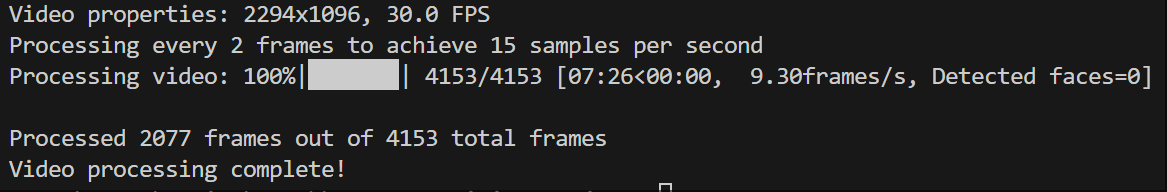
\includegraphics[width=0.8\linewidth]{sec/assets/original_command.png}
	 \caption{Original run with the naive pipeline: processing time was 7m26s.}
	 \label{fig:original_command}
\end{figure}

We tested multiple video resolutions to optimize processing speed. Our experiments showed that while high-resolution videos are not essential for effective face and emotion detection, excessively low resolution leads to detection failures. Testing demonstrated that 480P provided the optimal balance between accuracy and performance, reducing processing time to just 1m38s (Figure \ref{fig:480P_command}). Based on these findings, we implemented automatic resolution adjustment to approximately 480P for all subsequent experiments.
\begin{figure}[!htb]
	\centering
	 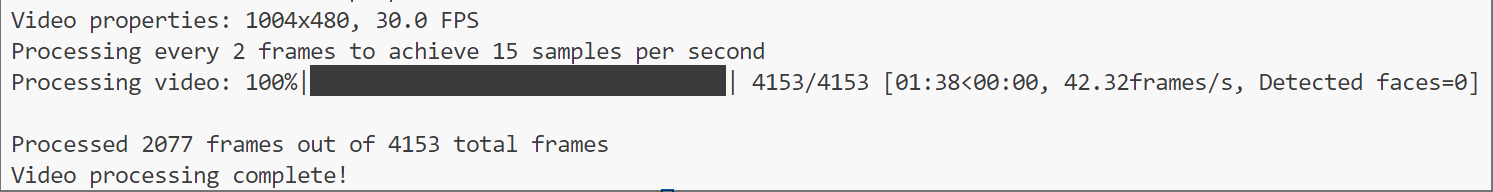
\includegraphics[width=0.8\linewidth]{sec/assets/480P_command.png}
	 \caption{The 480P video required only 1m38s to process.}
	 \label{fig:480P_command}
\end{figure}

A key optimization involved implementing local detection: examining only the area surrounding the previous frame's face location, unless no face was detected. We tested various padding sizes, with pad dynamically defined as: $\text{pad} = \max(30, \text{int}(\text{p} \cdot \max(\text{face\_width}, \text{face\_height})))$. Figure \ref{fig:pad_size} presents our experimental results. We selected p=1.0 as the optimal trade-off between processing speed and detection accuracy.

We also implemented dynamic resolution adjustment based on face size. When the face-to-image size ratio fell below a threshold (while maintaining sufficient resolution of at least 96$\times$96 pixels for reliable emotion detection), we downscaled the image by a factor of 2. The scaling parameter reset whenever no face was detected in the previous frame. With p=1.0, this optimization further reduced processing time to 1m10s (Figure \ref{auto_face_command}), showing promising potential for real-time applications.

\begin{figure}[!htb]
\centering
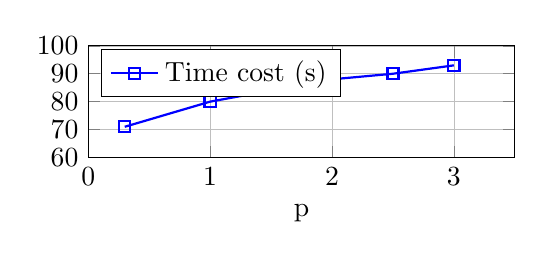
\begin{tikzpicture}
\begin{axis}[
	width=7cm,
	height=3cm,
	xlabel={p},
	ylabel={},
	xmin=0, xmax=3.5,
	ymin=60, ymax=100,
	xtick={0,1,2,3},
	ytick={60,70,80,90,100},
	legend pos=north west,
	grid=both,
	grid style={line width=.05pt, draw=gray!10},
	major grid style={line width=.2pt,draw=gray!50}
]
\addplot[mark=square,blue,thick] coordinates {
	(0.3,71)
	(1.0,80)
	(2.0,88)
		(2.5,90)
		(3.0,93)
};
\legend{Time cost (s)}
\end{axis}
\end{tikzpicture}
\caption{Processing time with different pad sizes. The pad size is dynamically defined as: $\text{pad} = \max(30, \text{int}(\text{p} \cdot \max(\text{face\_width}, \text{face\_height})))$. Global detection alone would require approximately 100s.}
\label{fig:pad_size}
\end{figure}

\begin{figure}[!htb]
	\centering
	 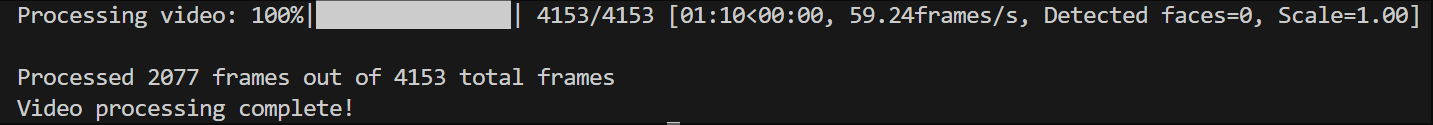
\includegraphics[width=0.8\linewidth]{sec/assets/auto_face_command.png}
	 \caption{Automatic face resolution adjustment reduced processing time to 1m10s.}
	 \label{auto_face_command}
\end{figure}

\subsection{Recognition Accuracy}
As mentioned previously, untrained humans achieve approximately 40\% accuracy in emotion recognition, while trained humans reach about 60\%. Our model achieved 62\% accuracy, comparable to trained human performance.

\subsection{Result Demonstration}
Figure \ref{fig:jg_exp} demonstrates our emotion detection system in action. The model successfully identified both faces and correctly classified their emotions as "happy."

\begin{figure}[!htb]
	\centering
	 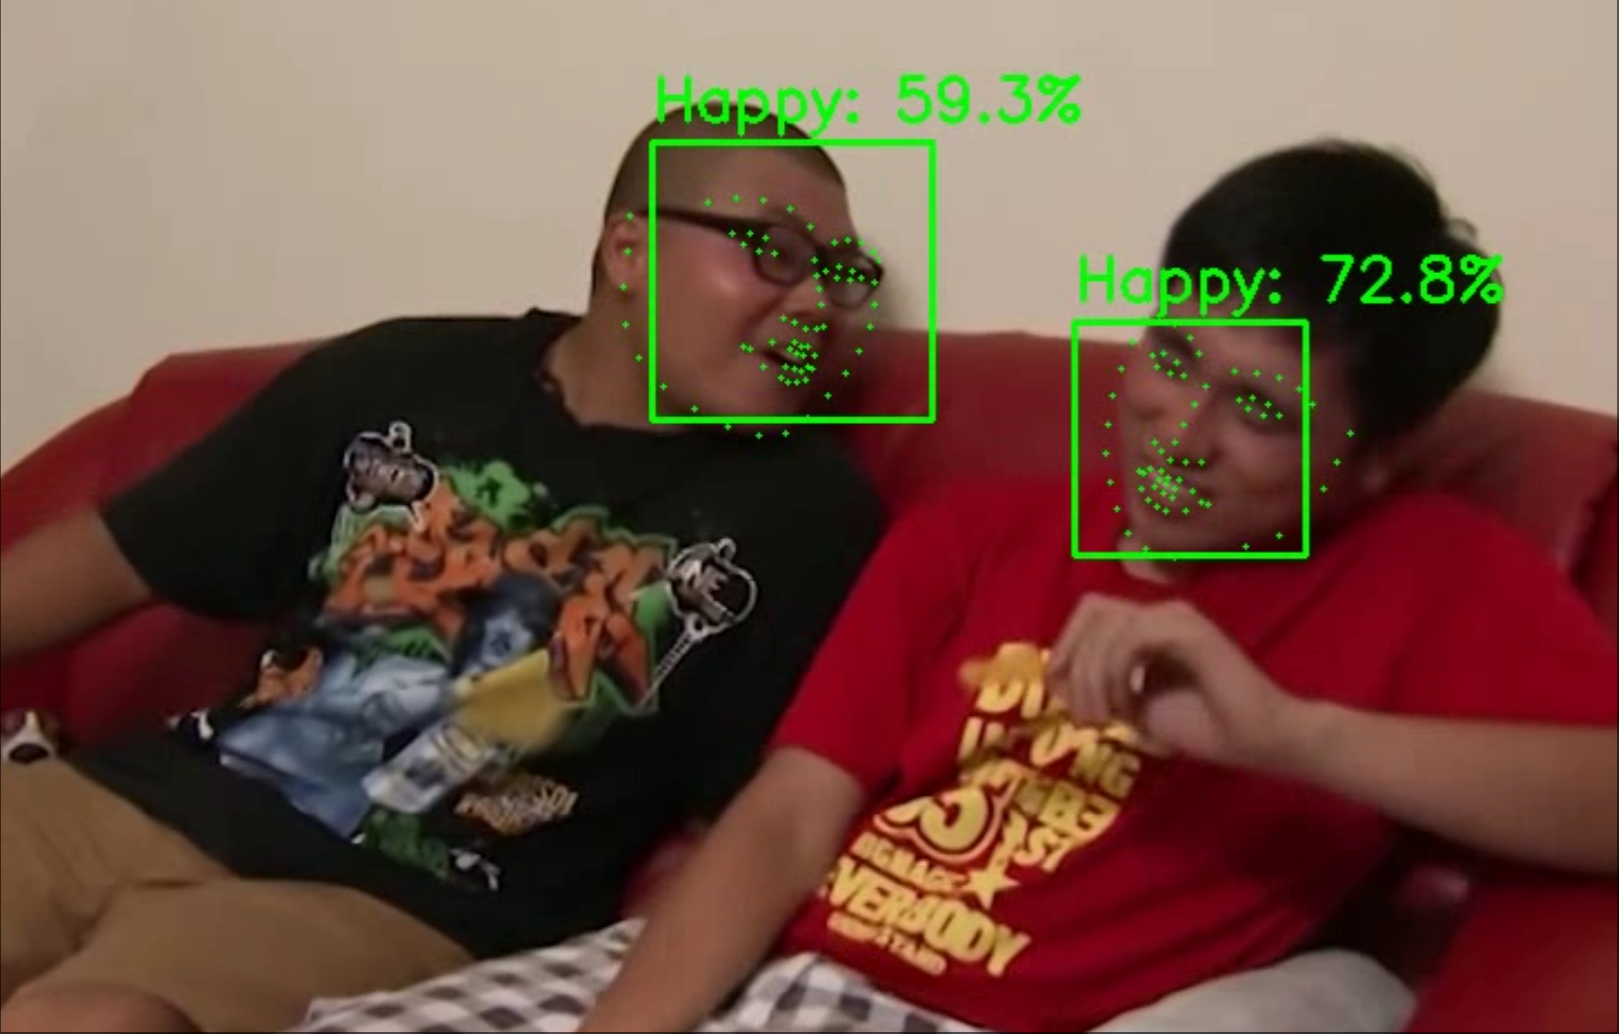
\includegraphics[width=0.6\linewidth]{sec/assets/jg_exp.png}
	 \caption{Example of emotion detection. The model successfully recognizes two faces and correctly identifies both emotions as "happy."}
	 \label{fig:jg_exp}
\end{figure}

The video processing time of approximately 1 minute and 10 seconds enabled analysis at nearly 24 frames per second, making it suitable for real-time applications.
